\documentclass[11pt]{beamer}
\usetheme{Berkeley}
\usecolortheme{wolverine}

\usepackage[utf8]{inputenc}
\usepackage[english]{babel}
\usepackage{csquotes}
\usepackage{amsmath}
\usepackage{amsfonts}
\usepackage{amssymb}
\usepackage{graphicx}

\author{Mario Tambos}

\title{Improving Spike Sorting}

\subtitle{(untangling the brain's cables)}

\institute{M.sc. Computer Science \\ TU Berlin}

\date{\today}

\begin{document}
	\maketitle
	\begin{frame}
		\section{What is Spike sorting?}
		\frametitle{What is Spike sorting?}
		According to Wikipedia:
		\begin{quote}
			Spike sorting refers to the process of assigning spikes to different neurons.
		\end{quote}
	\end{frame}
	\begin{frame}
		\section{Spike sorting's applications}
		\frametitle{Spike sorting's applications}
		\begin{itemize}
			\item Prosthetics.
			\begin{itemize}
				\item Missing limbs.
				\item Locked-in syndrome.
				\item Remote presence.
			\end{itemize}
			\item Disease diagnosis.
			\begin{itemize}
				\item Detect abnormal firing patterns.
			\end{itemize}
			\item Research.
			\begin{itemize}
				\item Pinpoint certain neurons as triggers for some action.
			\end{itemize}
		\end{itemize}
	\end{frame}
	\begin{frame}
		In other words: \textbf{HUGE} impact!
	\end{frame}
	\begin{frame}
		\section{What does the problem look like?}
		\frametitle{What does the problem look like?}
		\begin{itemize}
			\item (Multi-)Electrodes are inserted in live animals (in-vivo) or cultures of brain cells (in-vitro) during experiments
		\end{itemize}
		\begin{figure}[p]
			\centering
			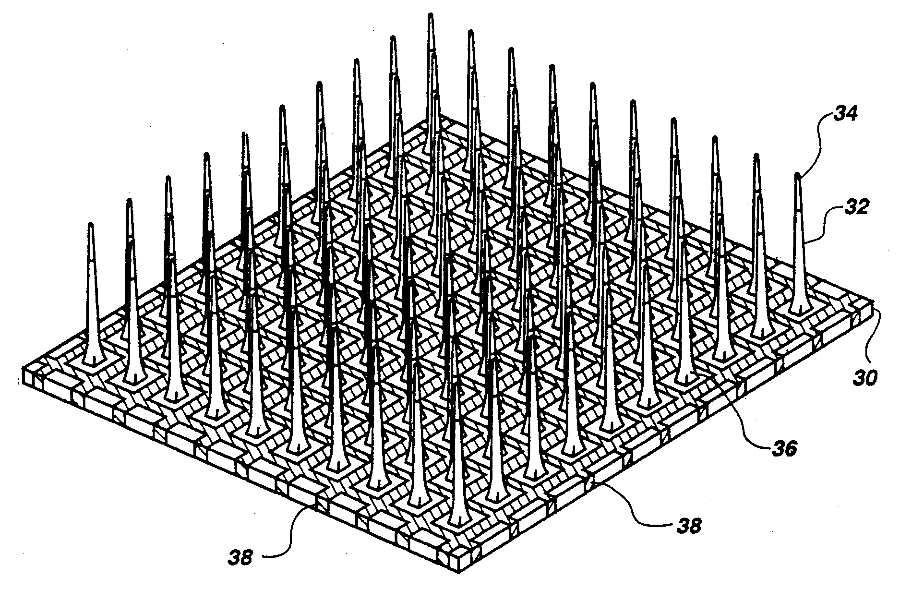
\includegraphics[scale=0.4]{images/Utah_array_pat5215088.jpg}
			\caption{Electrode array (Source: \url{http://scholarpedia.org/})}
		\end{figure}
	\end{frame}
	\begin{frame}
		\begin{itemize}
			\item Electrical readings are taken from the brain cells via the electrodes.
		\end{itemize}
		\begin{figure}[p]
			\centering
			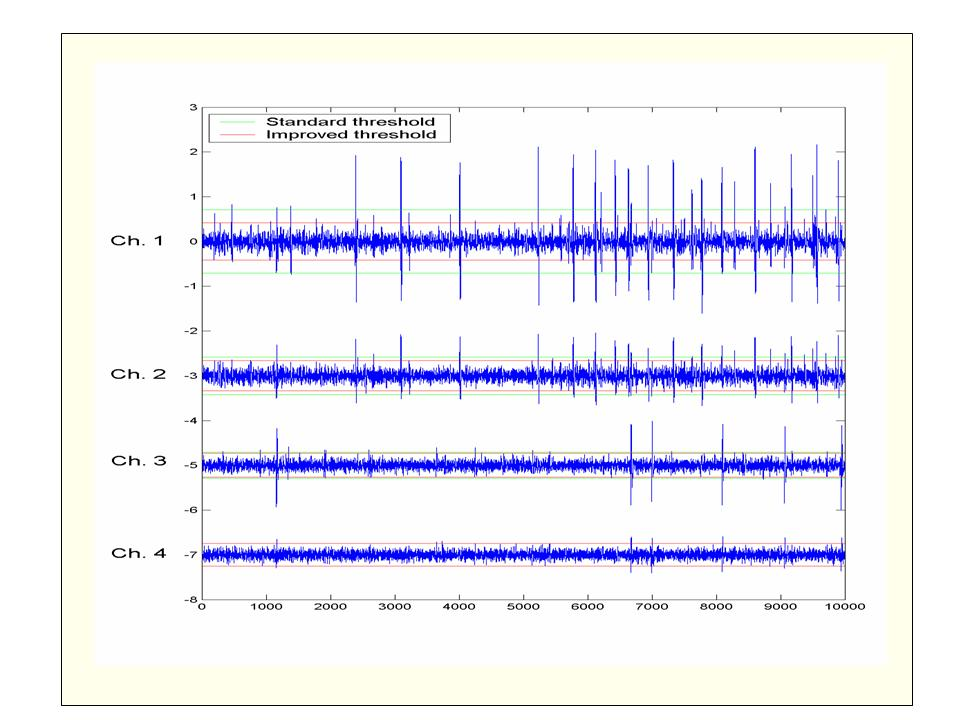
\includegraphics[scale=0.25]{images/QQ_Fig6.jpg}
			\caption{Electrode readings (Source: \url{http://scholarpedia.org/})}
		\end{figure}
	\end{frame}
	\begin{frame}
		\begin{itemize}
			\item Some process is applied to the input signal(s) [$\Leftarrow$ spike sorting proper].
		\end{itemize}
		\begin{figure}[p]
			\centering
			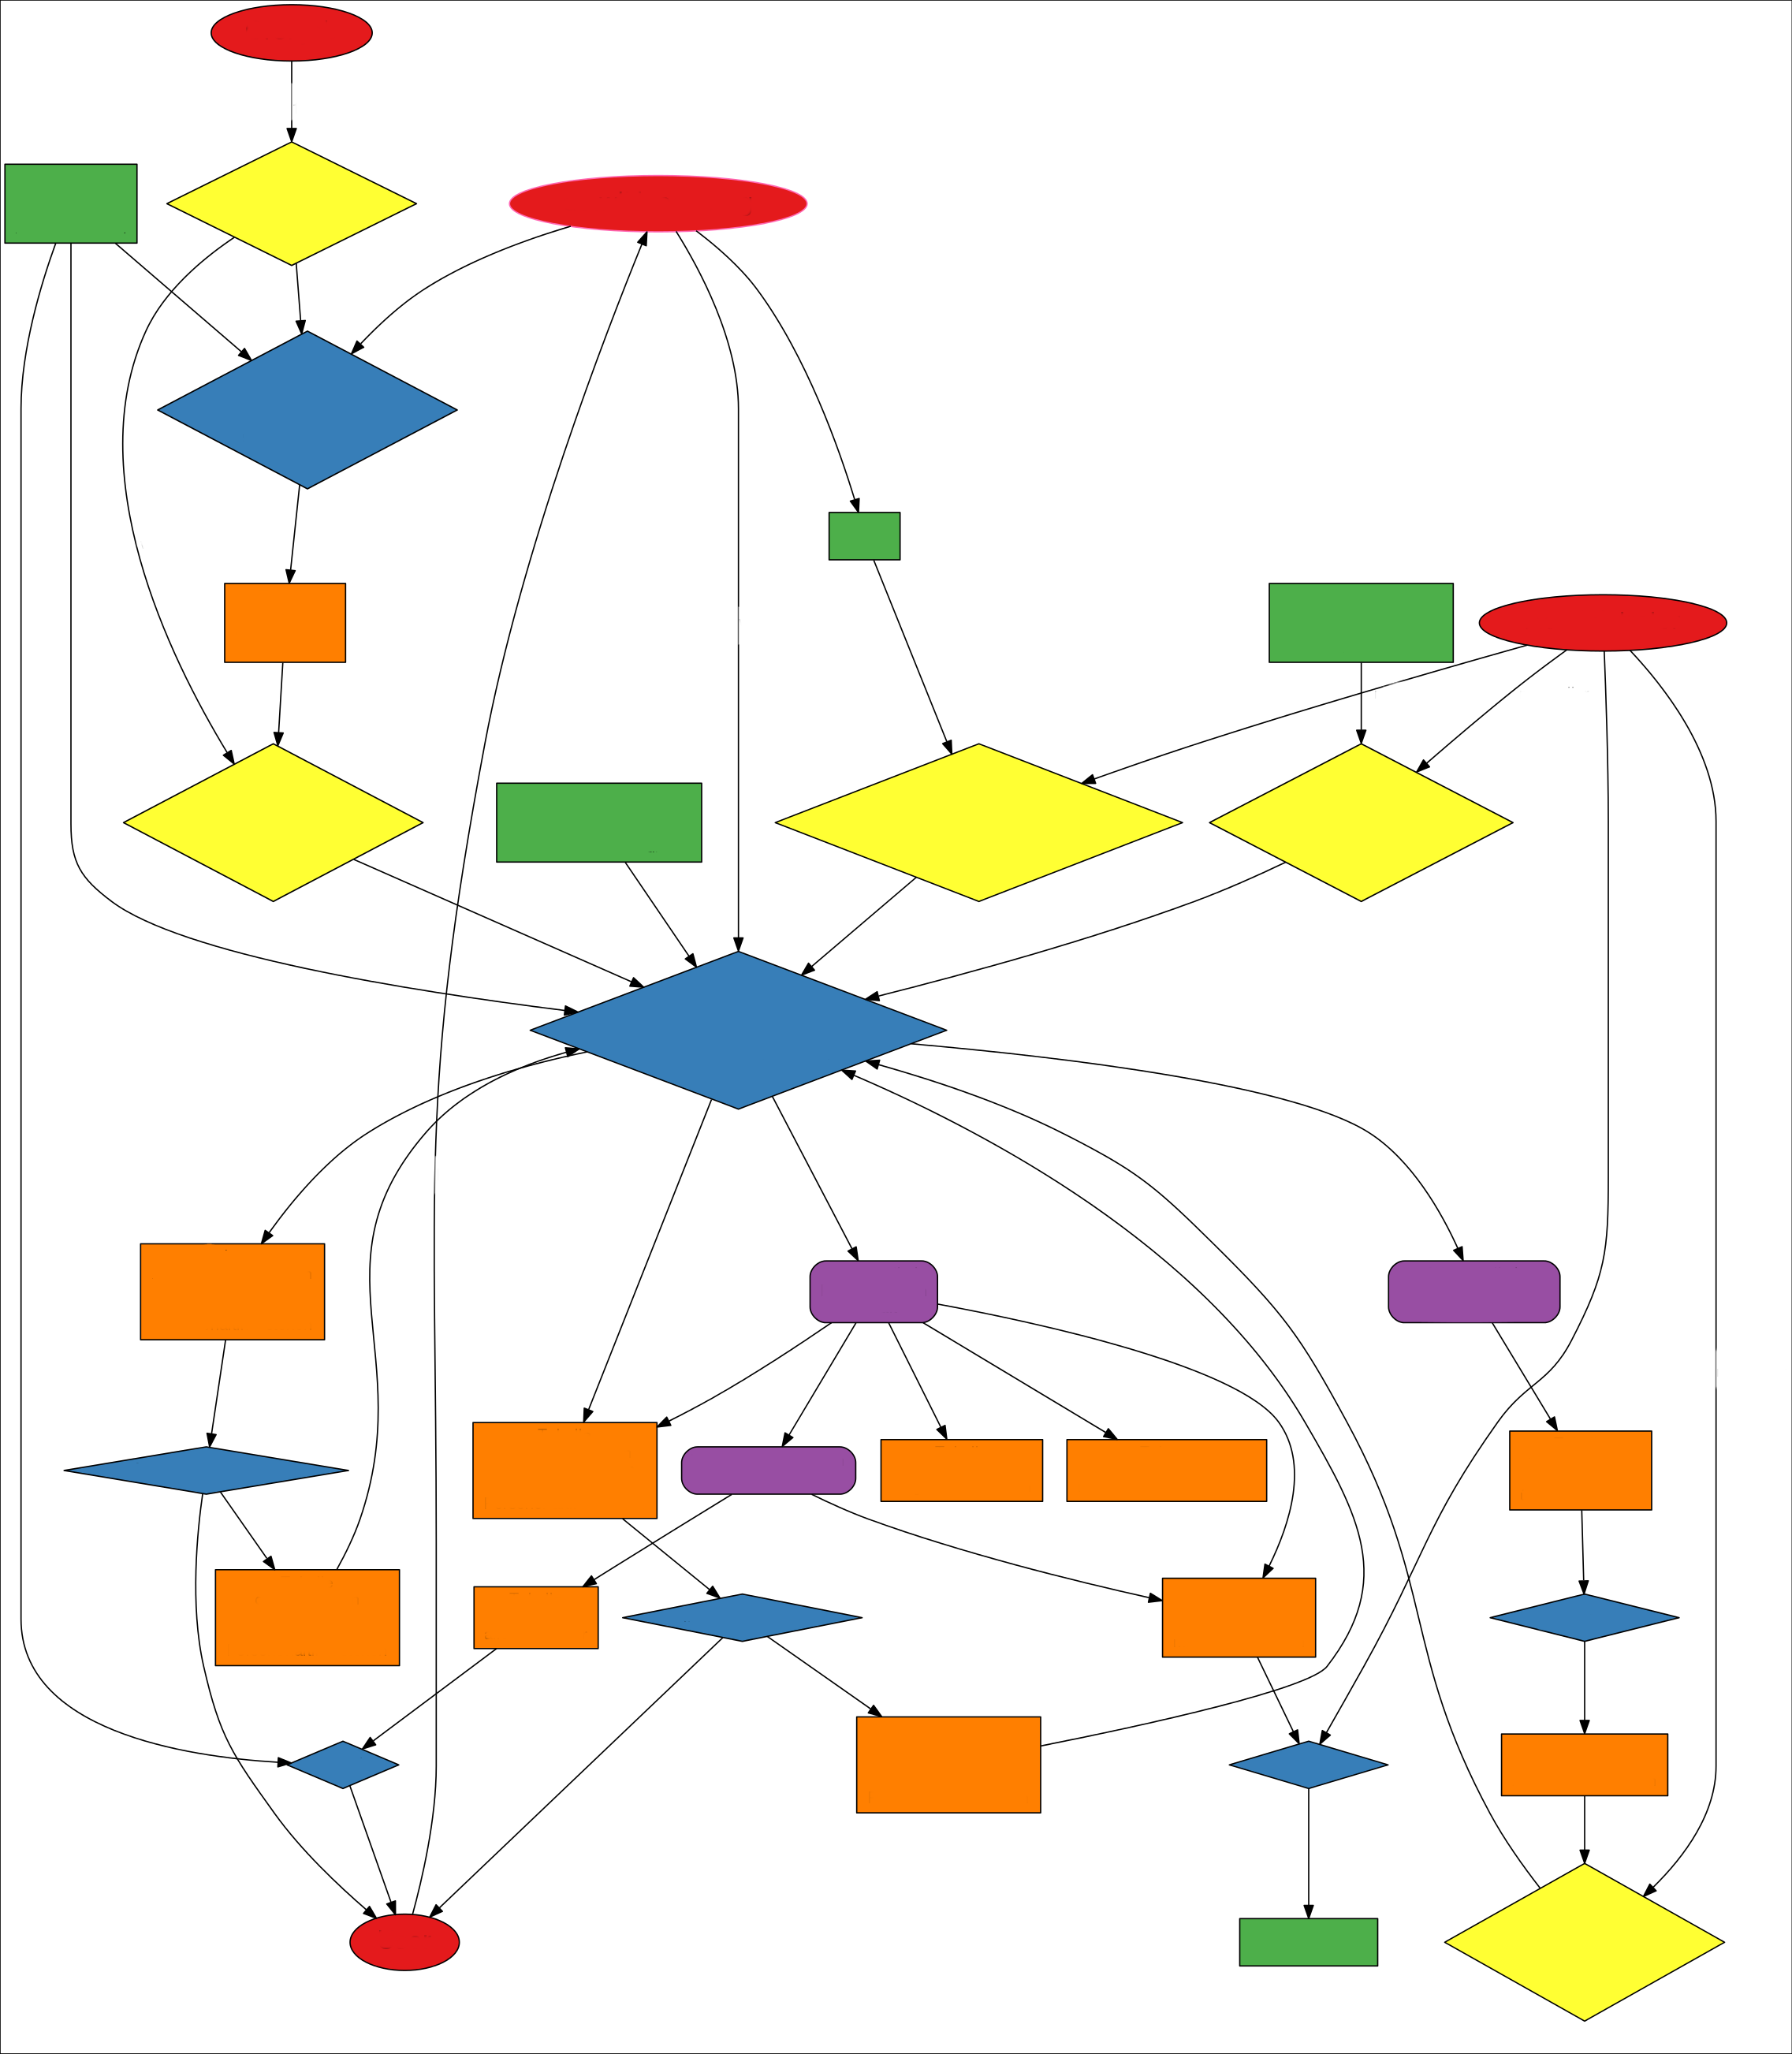
\includegraphics[scale=0.05]{images/Workflow_Personendaten_Wartung.png}
			\caption{Preprocessing and sorting procedure(s) (Source: \url{http://wikimedia.org/})}
		\end{figure}
	\end{frame}
	\begin{frame}
		\begin{itemize}
			\item ... And we identify what neuron caused which spike.
		\end{itemize}
		\begin{figure}[p]
			\centering
			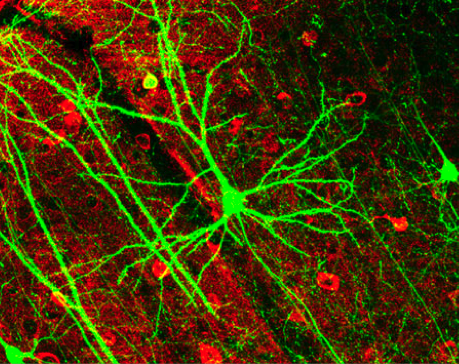
\includegraphics[scale=0.3]{images/GFPneuron.png}
			\caption{The culprit (Source: \url{http://wikimedia.org/})}
		\end{figure}
	\end{frame}
	\begin{frame}
		\begin{figure}[p]
			\centering
			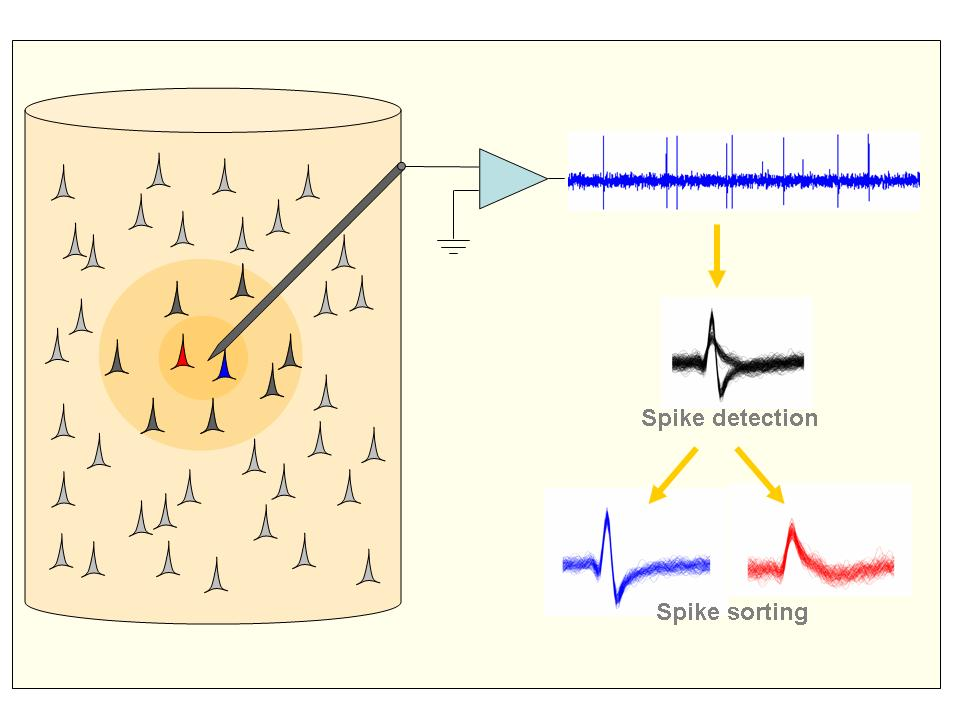
\includegraphics[scale=0.3]{images/QQ_Fig1.jpg}
			\caption{Spike sorting in a nutshell (Source: \url{http://scholarpedia.org/})}
		\end{figure}
	\end{frame}
	\begin{frame}
		\section{Challenges}
		\frametitle{Challenges}
		\begin{itemize}
			\item Difficult to evaluate the methods' performance.
			\begin{itemize}
				\item No ground truth in the in-vivo case.
			\end{itemize}
			\item Spikes sometimes overlap.
			\item Some common assumptions do not always hold.
			\begin{itemize}
				\item A neuron's spikes have all the same form.
				\item All neurons produce different spike's forms.
				\item The spikes' form is time-invariant.
			\end{itemize}
		\end{itemize}
	\end{frame}
	\begin{frame}
		\begin{itemize}
			\item We're basically trying to identify the source of a signal by sticking a rod into a mess of cables.
		\end{itemize}
		\begin{figure}[p]
			\centering
			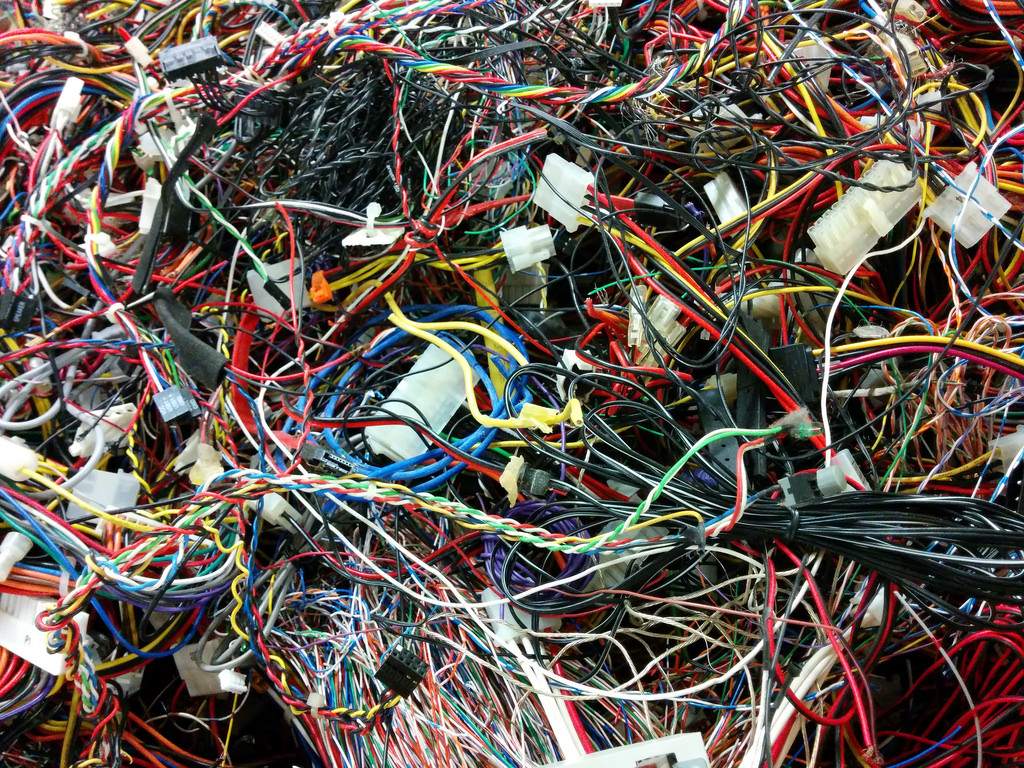
\includegraphics[scale=0.15]{images/tangled_cables.jpg}
			\caption{A methaphoric brain (Source: \url{https://www.flickr.com/photos/doctorow})}
		\end{figure}
	\end{frame}
	\begin{frame}
		\section{Project's Objectives}
		\frametitle{Project's Objectives}
		The project aims to have a working spike sorting pipeline.

		The main tasks are:
		\begin{itemize}
			\item Research current state-of-the-art.
			\item Implement one or more likely candidates, e.g.:
			\begin{itemize}
				\item Signal filters.
				\item Probabilistic models.
				\item Artificial neural networks.
			\end{itemize}
			\item Evaluate performance using synthetic or in-vitro recordings.
			\item Write findings in a research paper.
		\end{itemize}
	\end{frame}
	\begin{frame}
		\section{END}
		\frametitle{END}
		THANK YOU!
	\end{frame}
	
\end{document}